\tableofcontents
\section{BulletInterface}
\subsection{接口类}
\subsection{BWAPI::BulletInterface继承图}
\begin{figure}[H]
    \centering
    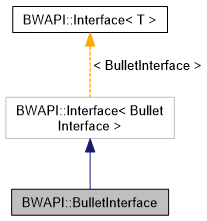
\includegraphics[width=0.4\textwidth]{figures/BulletInterface继承图.png}
\end{figure}
\subsubsection{公共成员函数}
\begin{codebox}[公共成员函数]
virtual bool exists () const =0
virtual double getAngle () const =0
virtual int getID () const =0
virtual Player getPlayer () const =0
virtual Position getPosition () const =0
virtual int getRemoveTimer () const =0
virtual Unit getSource () const =0
virtual Unit getTarget () const =0
virtual Position getTargetPosition () const =0
virtual BulletType getType () const =0
virtual double getVelocityX () const =0
virtual double getVelocityY () const =0
virtual bool isVisible (Player player=nullptr) const =0
\end{codebox}
\subsubsection{详细描述}
接口对象,表示从攻击中生成的子弹或飞弹。\par
Bullet 接口允许你检测子弹、飞弹以及其他类型的非近战攻击或特殊能力,这些通常是人类玩家通过视觉可以看到的(例如潜伏者的地刺或女皇的寄生飞虫)。这使得 AI 可以更快地对不可避免的后果做出反应。\par
例如,你可以命令medic提前治疗即将被锁定的unit,以补偿延迟并尽量减少其影响。除非你能够通过 Bullet 类检测到锁定飞弹,否则你无法完全知道哪个unit将被锁定。\par
Bullet 对象在被销毁后会被重新使用,但当它代表一个新的 Bullet 时,其 ID 会被更新。\par
如果禁用了   Flag::CompleteMapInformation  ,那么只有可见的 Bullet 才能被访问。否则,如果启用了   Flag::CompleteMapInformation  ,那么游戏中所有的 Bullet 都可以被访问。\par
\begin{refer}
    \begin{itemize}
        \item Game::getBullets
        \item BulletInterface::exists
    \end{itemize}
\end{refer}

\subsubsection{成员函数文档}

\begin{tcolorbox}[colback=white, colframe=black!60!white, title=getID(), arc=0mm]
\begin{minted}[frame=none]{cpp}
virtual int BWAPI::BulletInterface::getID() const
\end{minted}
获取当前子弹的唯一标识符。
\begin{return}
    \begin{itemize}
            \item int:子弹标识符
    \end{itemize}
\end{return}
\end{tcolorbox}

\begin{tcolorbox}[colback=white, colframe=black!60!white, title=exists(), arc=0mm]
\begin{minted}[frame=none]{cpp}    
virtual bool BWAPI::BulletInterface::exists() const
\end{minted}
检查Bullet是否存在于BWAPI player的视野中。
\begin{return}
    \begin{itemize}
        \item \texttt{bool}:子弹存在或可见(true) / 已被销毁或超出作用范围(false)
    \end{itemize}
\end{return}
如果禁用了  Flag::CompleteMapInformation  ,并且一个  Bullet  不可见,那么无论该bullet是否真实存在,返回值都将为  false  。这是因为对于不可见的敌方bullet,AI无法获取任何状态信息。\par
如果启用了  Flag::CompleteMapInformation  ,那么这个函数对于所有  Bullet  信息都是准确的。
\begin{refer}
    \begin{itemize}
        \item isVisible
        \item UnitInterface::exists
    \end{itemize}
\end{refer}
\end{tcolorbox}

\begin{tcolorbox}[colback=white, colframe=black!60!white, title=getPlayer(), arc=0mm]
    \begin{minted}[frame=none]{cpp}
virtual Player BWAPI::BulletInterface::getPlayer() const
    \end{minted}
    获取拥有该Bullet的Player接口对象。
    \begin{return}
        \begin{itemize}
            \item \texttt{Player}:拥有该Bullet的Player接口对象 / 无法访问该Bullet的Player对象(nullptr)
        \end{itemize}
    \end{return}
\end{tcolorbox}


\begin{tcolorbox}[colback=white, colframe=black!60!white, title=getType(), arc=0mm]
    \begin{minted}[frame=none]{cpp}
virtual BulletType BWAPI::BulletInterface::getType() const
    \end{minted}
    获取当前Bullet的类型。
    \begin{return}
        \begin{itemize}
            \item \texttt{BulletType}:Bullet类型 / Bullet无法访问 (BulletTypes::Unknown)
        \end{itemize}
    \end{return}
\end{tcolorbox}

\begin{tcolorbox}[colback=white, colframe=black!60!white, title=getSource(), arc=0mm]
    \begin{minted}[frame=none]{cpp}
virtual Unit BWAPI::BulletInterface::getSource() const
    \end{minted}
    获取发射这颗Bullet的Unit接口对象。
    \begin{return}
        \begin{itemize}
            \item \texttt{Unit}:拥有该Bullet的Unit接口对象 / 无法识别或访问发射源 (nullptr)
        \end{itemize}
    \end{return}
    \begin{refer}
        \begin{itemize}
            \item getTarget
        \end{itemize}
    \end{refer}
\end{tcolorbox}

\begin{tcolorbox}[colback=white, colframe=black!60!white, title=getPosition(), arc=0mm]
    \begin{minted}[frame=none]{cpp}
virtual Position BWAPI::BulletInterface::getPosition() const
    \end{minted}
    获取Bullet的当前位置。
    \begin{return}
        \begin{itemize}
            \item \texttt{Position}:子弹当前的位置 / 子弹无法访问 (Positions::Unknown)
        \end{itemize}
    \end{return}
    \begin{refer}
        \begin{itemize}
            \item getTargetPosition
        \end{itemize}
    \end{refer}
\end{tcolorbox}

\begin{tcolorbox}[colback=white, colframe=black!60!white, title=getAngle(), arc=0mm]
    \begin{minted}[frame=none]{cpp}
virtual double BWAPI::BulletInterface::getAngle() const
    \end{minted}
    获取Bullet的朝向方向。如果angle为0,则Bullet朝向为right。
    \begin{return}
        \begin{itemize}
            \item double:Bullet的angle / Bullet无法访问 (0.0)
        \end{itemize}
    \end{return}
    \begin{refer}
        \begin{itemize}
            \item getTargetPosition
        \end{itemize}
    \end{refer}
\end{tcolorbox}

\begin{tcolorbox}[colback=white, colframe=black!60!white, title=getVelocityX(), arc=0mm]
    \begin{minted}[frame=none]{cpp}
virtual double BWAPI::BulletInterface::getVelocityX() const
    \end{minted}
    获取Bullet在X轴方向上的速度分量。
    \begin{return}
        \begin{itemize}
            \item double:Bullet每frame在X轴方向上移动的pixel数 / Bullet无法访问 (0.0)
        \end{itemize}
    \end{return}
    \begin{refer}
        \begin{itemize}
            \item getVelocityY
            \item getAngle
        \end{itemize}
    \end{refer}
\end{tcolorbox}

\begin{tcolorbox}[colback=white, colframe=black!60!white, title=getVelocityY(), arc=0mm]
    \begin{minted}[frame=none]{cpp}
virtual double BWAPI::BulletInterface::getVelocityY() const
    \end{minted}
    获取Bullet在Y轴方向上的速度分量。
    \begin{return}
        \begin{itemize}
            \item double:Bullet每frame在Y轴方向上移动的pixel数 / Bullet无法访问 (0.0)
        \end{itemize}
    \end{return}
    \begin{refer}
        \begin{itemize}
            \item getVelocityX
            \item getAngle
        \end{itemize}
    \end{refer}
\end{tcolorbox}

\begin{tcolorbox}[colback=white, colframe=black!60!white, title=getTarget(), arc=0mm]
    \begin{minted}[frame=none]{cpp}
virtual Unit BWAPI::BulletInterface::getTarget() const
    \end{minted}
    获取Bullet的目标Unit接口对象。
    \begin{return}
        \begin{itemize}
            \item \texttt{Unit}:存在目标Unit / Bullet目标Unit无法访问,或者Bullet的目标是ground,或者Bullet本身无法访问 (nullptr)
        \end{itemize}
    \end{return}
    \begin{refer}
        \begin{itemize}
            \item getTargetPosition
            \item getSource
        \end{itemize}
    \end{refer}
\end{tcolorbox}

\begin{tcolorbox}[colback=white, colframe=black!60!white, title=getTargetPosition(), arc=0mm]
    \begin{minted}[frame=none]{cpp}
virtual Position BWAPI::BulletInterface::getTargetPosition() const
    \end{minted}
    获取Bullet的目标位置。
    \begin{return}
        \begin{itemize}
            \item \texttt{Position}:Bullet的飞行目标位置 / Bullet无法访问 (Positions::Unknown)
        \end{itemize}
    \end{return}
    \begin{refer}
        \begin{itemize}
            \item getTarget
            \item getPosition
        \end{itemize}
    \end{refer}
\end{tcolorbox}

\begin{tcolorbox}[colback=white, colframe=black!60!white, title=getRemoveTimer(), arc=0mm]
    \begin{minted}[frame=none]{cpp}
virtual int BWAPI::BulletInterface::getRemoveTimer() const
    \end{minted}
    获取Bullet的剩余寿命。Bullet不是永久对象,通常有一个有限的寿命,以frame为单位测量。
    \begin{return}
        \begin{itemize}
            \item int:Bullet自毁前剩余的frame数 / Bullet无法访问 (0)
        \end{itemize}
    \end{return}
    \begin{refer}
        \begin{itemize}
            \item getTarget
            \item getPosition
        \end{itemize}
    \end{refer}
\end{tcolorbox}

\begin{tcolorbox}[colback=white, colframe=black!60!white, title=isVisible(), arc=0mm]
    \begin{minted}[frame=none]{cpp}
virtual bool BWAPI::BulletInterface::isVisible(Player player = nullptr) const
    \end{minted}
    获取Bullet的可见性状态。
    \begin{parameter}
        \begin{itemize}
            \item \texttt{player}(可选):如果指定了这个参数,则检查该player是否能看到这颗bullet。如果未指定此参数,则使用默认值nullptr,此时会检查BWAPI player是否能看到这颗bullet。
        \end{itemize}
    \end{parameter}
    \begin{note}
        如果player是nullptr,并且Broodwar->self()也是nullptr,则通过检查是否有其他player能看到这颗bullet来确定其可见性。
    \end{note}
    \begin{return}
        \begin{itemize}
            \item \texttt{bool}:指定player可以看到这颗bullet (true) / 指定player看不到这颗bullet (false)
        \end{itemize}
    \end{return}
\end{tcolorbox}